\documentclass{article}

% \usepackage{nips_2017}
\usepackage[final]{nips_2017}

\usepackage{polski}
\usepackage[utf8]{inputenc} % allow utf-8 input
\usepackage[T1]{fontenc}    % use 8-bit T1 fonts
% \usepackage{hyperref}       % hyperlinks
% \usepackage{url}            % simple URL typesetting
% \usepackage{booktabs}       % professional-quality tables
% \usepackage{amsfonts}       % blackboard math symbols
% \usepackage{nicefrac}       % compact symbols for 1/2, etc.
% \usepackage{microtype}      % microtypography
% \usepackage[section]{placeins}
\usepackage{graphicx}
\usepackage{interval}
\usepackage{float}
% \usepackage{subcaption}
\usepackage{subfig}

\title{Ćwiczenie 2 – Klasyfikacja obrazów przy pomocy płytkiej sieci jednokierunkowej} 
\author{Michał Kajstura}


\begin{document}

\maketitle

\tableofcontents
\raggedbottom
\pagebreak

\section{Plan eksperymentów}
\subsection{Cel}
Celem przeprowadzonych eksperymentów było zapoznanie się z modelem
płytkiej sieci neuronowej (ang. \textit{Multilayer perceptron}),
który był trenowany za pomocą algorytmu propagacji wstecznej.
Zbadano wpływ hiperparametrów takich jak:
\begin{itemize}
  \item liczba neuronów w warstwie ukrytej
  \item współczynnik uczenia
  \item rozmiar paczki
  \item przedział, z którego inicjalizowane są wagi
  \item wybór funkcji aktywacji
\end{itemize}
Porównano wartości funkcji straty oraz dokładności (ang. \textit{accuracy}).

\subsection{Metodyka badań}
Przyjęto następujące wartości domyślne hiperparametrów:
\begin{itemize}
  \item liczba neuronów w warstwie ukrytej - $256$
  \item współczynnik uczenia - $0.001$
  \item rozmiar paczki - $128$
  \item przedział inicjalizacji wag - 0.05
  \item funkcja aktywacji - ReLU
\end{itemize}
Podczas każdego eksperymentu, uczenie sieci neuronowej odbywało się przez 90 epok.
Funkcją straty użytą podczas treningu sieci była entropia krzyżowa.
Wagi początkowe zostały zainicjalizowane z rozkładu normalnego
o $\mu = 0$ i $\sigma = 0.05$

\raggedbottom
\pagebreak
\section{Badania}
\subsection{Liczba neuronów w warstwie ukrytej}
Liczba neuronów jest hiperparametrem, który decyduje o złożoności modelu.
Modele o małej pojemności mogą nie być w stanie dostatecznie dopasować się do 
ciągu treningowego.

\begin{figure}[H]
  \centering
  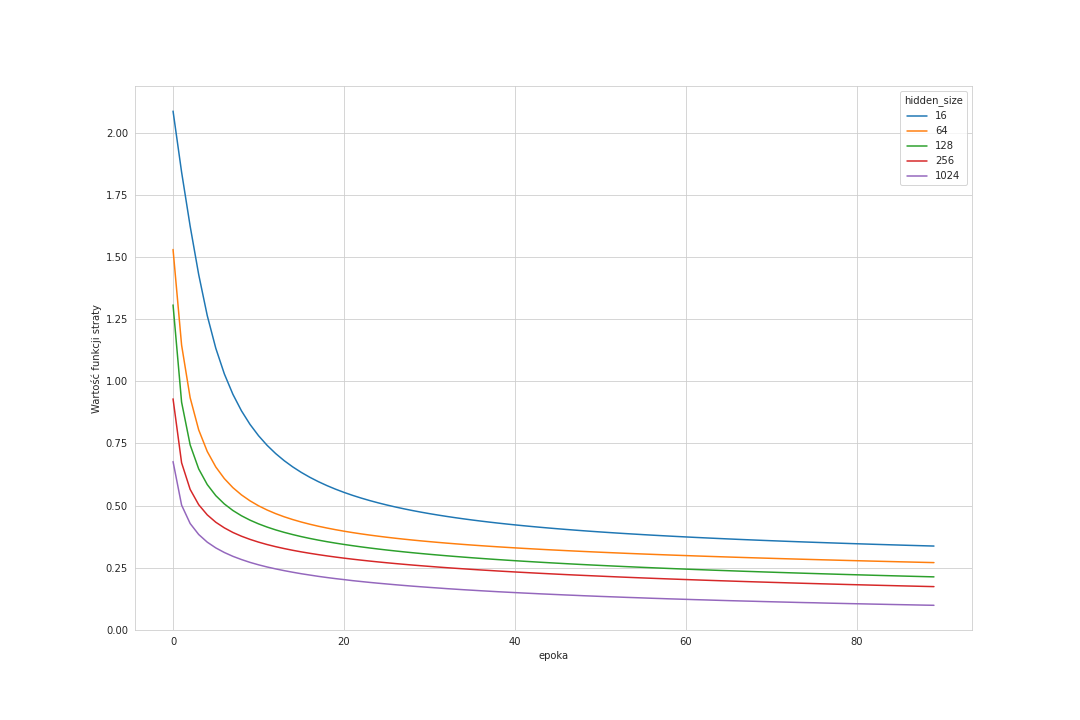
\includegraphics[width=\textwidth]{images/hidden_size_comp.png}
  \caption{Porównanie wpływu rozmiaru warstwy ukrytej na wartość funkcji straty}
\end{figure}
\begin{figure}[H]
    \centering
    \subfloat{{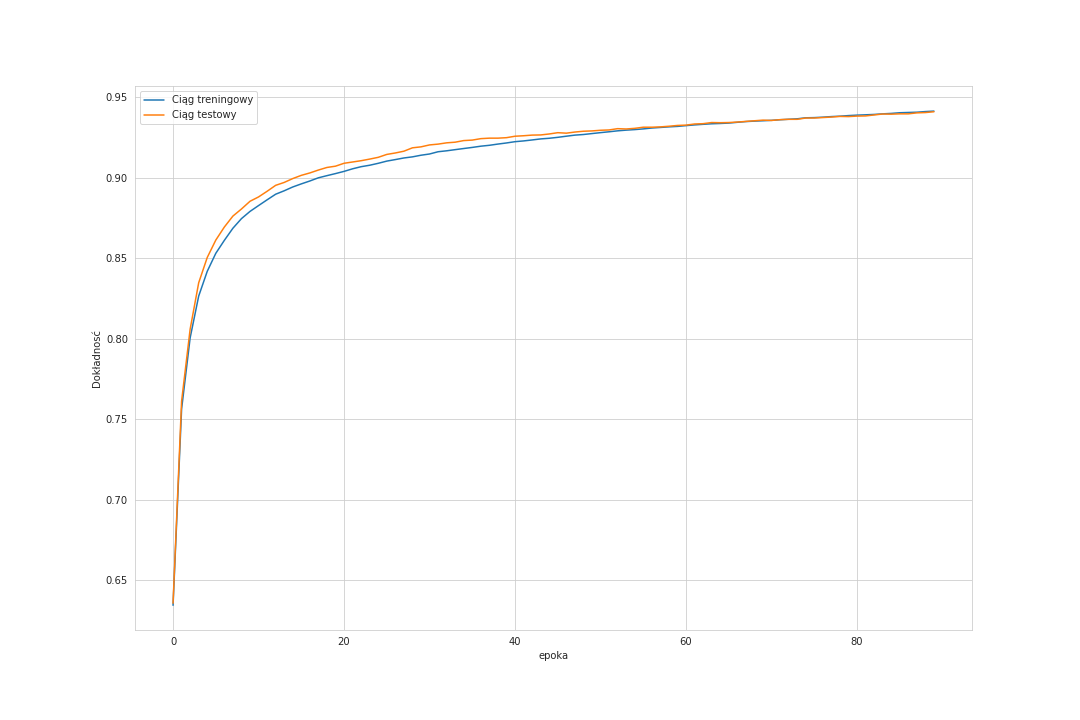
\includegraphics[width=0.45\textwidth]{images/hidden_size_128.png} }}
    \subfloat{{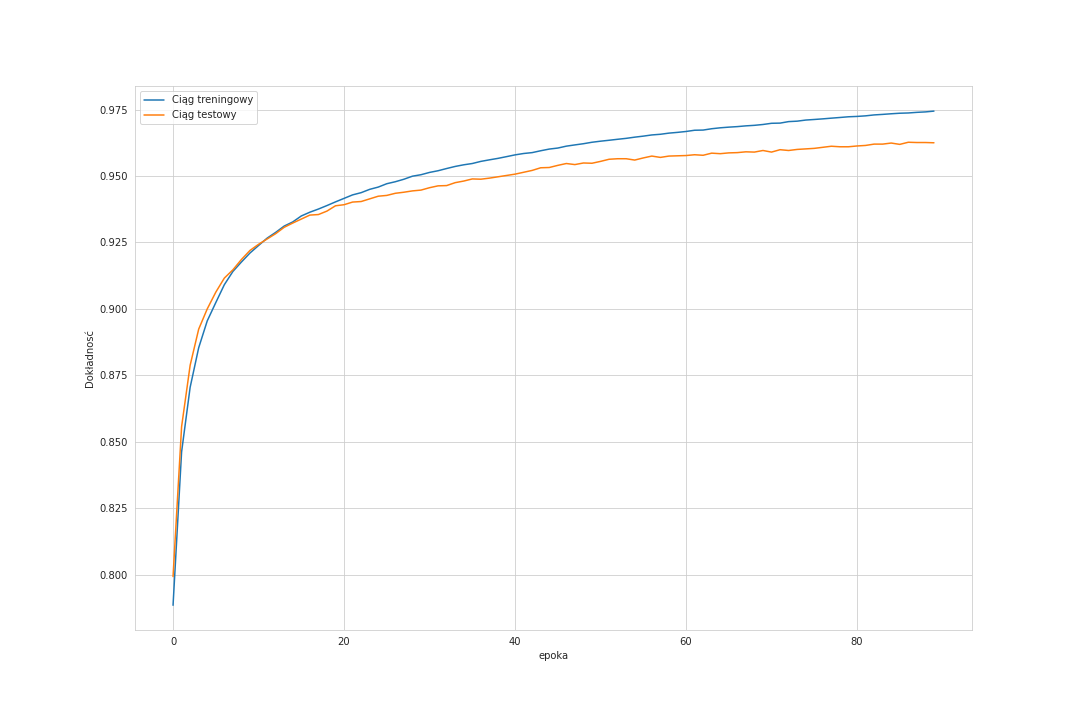
\includegraphics[width=0.45\textwidth]{images/hidden_size_1024.png} }}
  \caption{Porównanie dokładności modelu ze 128 i 1024 jednostkami ukrytymi}
\end{figure}

Wraz ze zwiększaniem rozmiaru modelu, wzrasta ryzyko 
przeuczenia (ang \textit{overfitting}).
Pomimo faktu, że podczas treningu dużego modelu wystąpiło przeuczenie przeuczenia, to i tak osiągnął on lepszy wynik, zarówno na ciągu treningowym, jak i testowym.


Warto pamiętać o tym, że ten hiperparametr ma wpływ na szybkość uczenia
oraz inferencji (mierzoną w sekundach).
\begin{figure}[H]
  \centering
  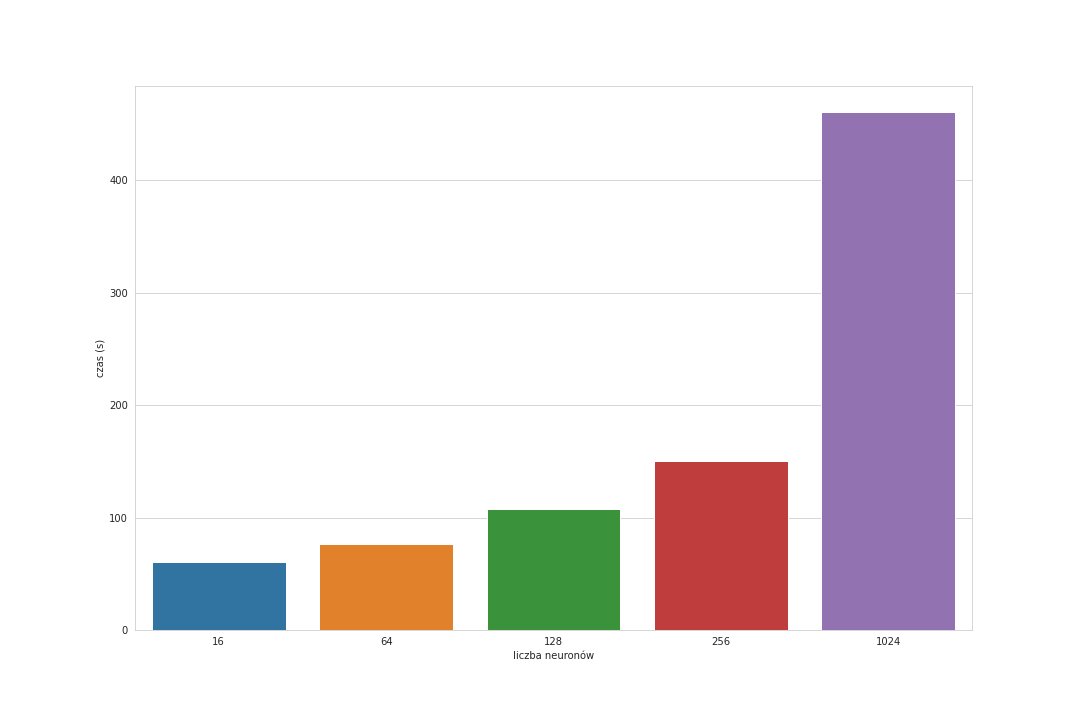
\includegraphics[width=0.8\textwidth]{images/hidden_size_times.png}
  \caption{Wpływ liczby neuronów na czas uczenia}
\end{figure}

\subsection{Współczynnik uczenia}
Współczynnik uczenia wpływa na szybkość uczenia algorytmu.
Zbyt mała wartość tego parametru oznacza wydłużenie czasu potrzebnego na uczenie.
Duża wartość może skutkować problemami ze zbieżnością.
Dobrą praktyką jest stosowanie harmonogramu (ang \textit{scheduling}), co pozwala na zaczęcie z duża wartością współczynnika uczenia i stopniowe zmniejszanie.
Podczas badań ta metoda nie zostałą wykorzystana, ponieważ utrudniałaby wyciągniecie wniosków na temat wpływu tego hiperparametru.

Przebieg uczenia był prawidłowy dla każdej przyjętej wartości współczynnika uczenia i nie dało się zaobserwować znacznych dewiacji.
\begin{figure}[H]
  \centering
  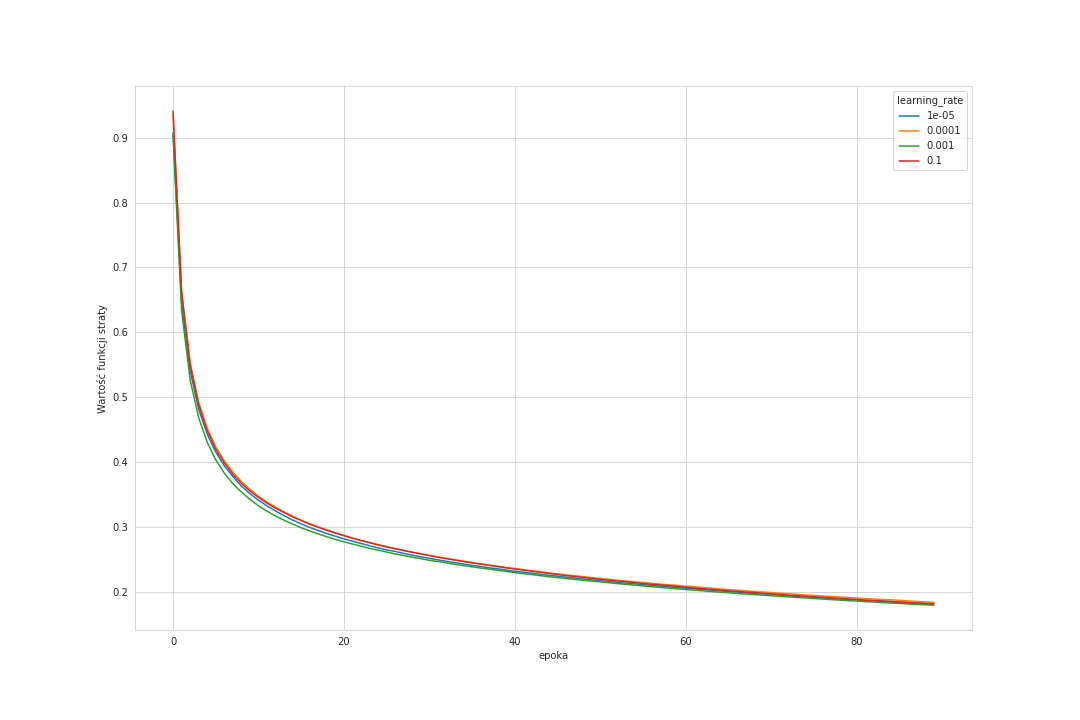
\includegraphics[width=0.8\textwidth]{images/learning_rate_comp.png}
  \caption{Wpływ współczynnika uczenia}
\end{figure}

\subsection{Rozmiar paczki}
Rozmiar paczki danych, na której jest wykonywana jedna iteracja ma duży wpływ na przebieg uczenia.
Im mniejsza paczka, tym więcej iteracji wykonywanych jest podczas jednej epoki.
Zbyt mały rozmiar paczki może skutkować dużym szumem i problemami ze zbieżnością.
Duży rozmiar paczki ma korzystny efekt na szybkość uczenia na kartach graficznych, ze względu na większe możliwości zrównoleglenia obliczeń.

Rozmiar paczki może mieć także wpływ na przeuczenie.
Szum wynikający z małego batcha czasami ma korzystny, regularyzujący wpływ.

\begin{figure}[H]
  \centering
  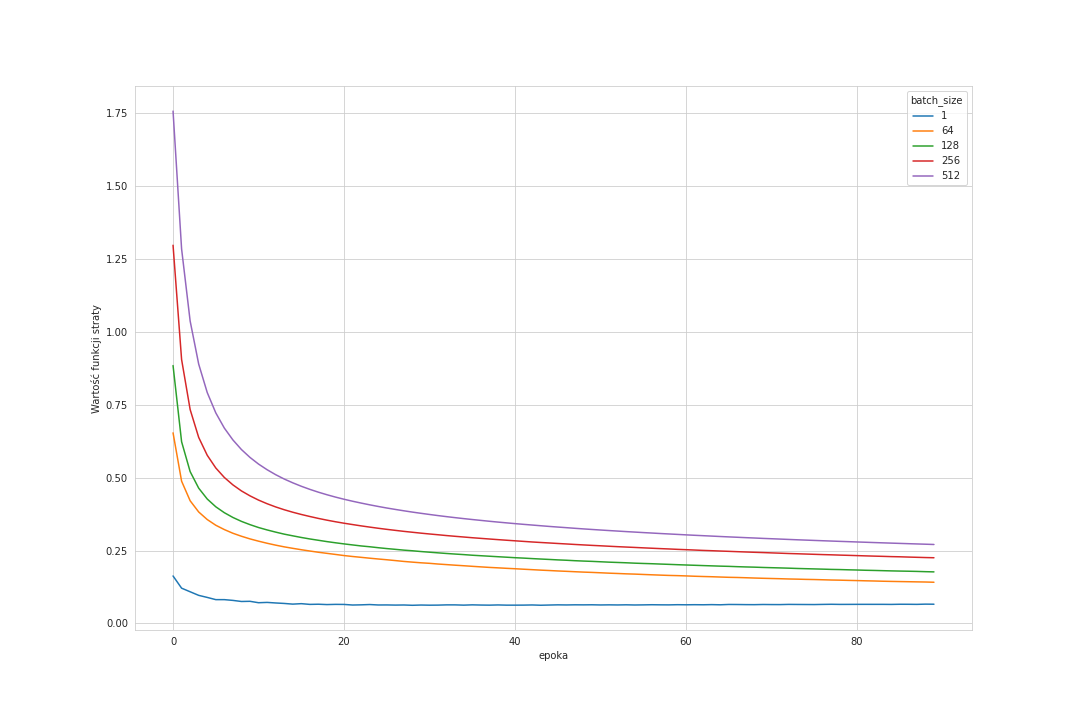
\includegraphics[width=\textwidth]{images/batch_size_comp.png}
  \caption{Wpływ wielkości paczki}
\end{figure}

Rozmiar batcha równy 1 oznaczał znacznie większą liczbę iteracji wykonanych podczas jednej epoki.
Z tego powodu można zaobserwować bardzo duże przeuczenie.

\begin{figure}[H]
  \centering
  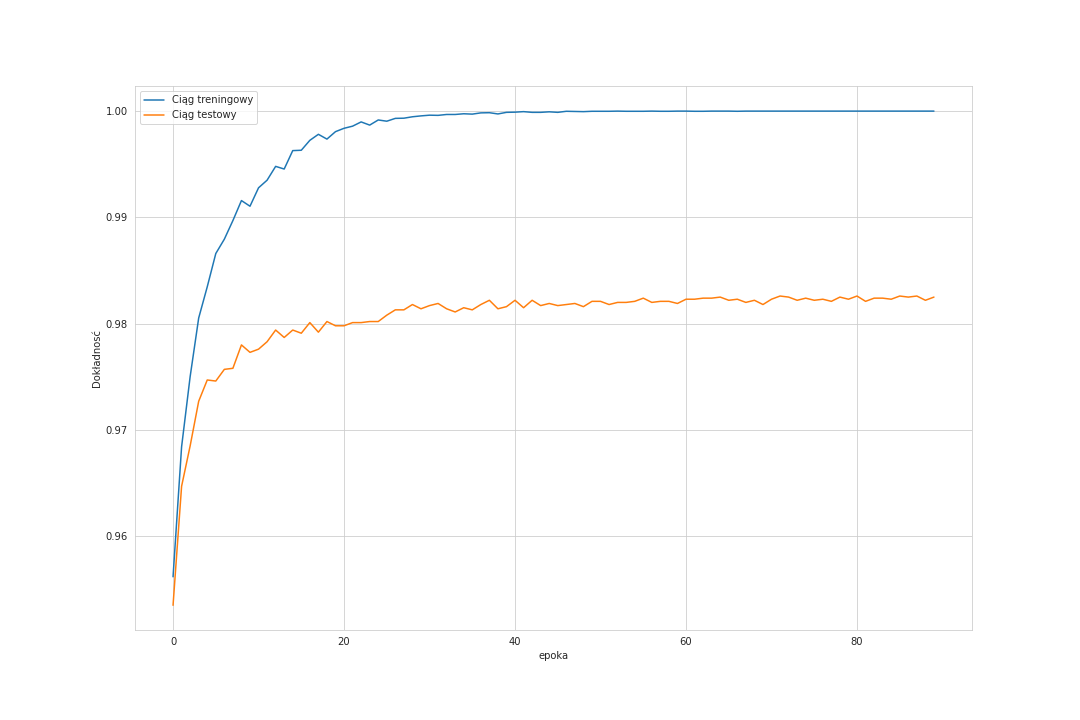
\includegraphics[width=\textwidth]{images/batch_size_accuracy.png}
  \caption{Rozmiar paczki równy 1}
\end{figure}

Trening przez stałą liczbę epok, przy użyciu bardzo małego rozmiaru paczki skutkował długim czasem uczenia.

\begin{figure}[H]
  \centering
  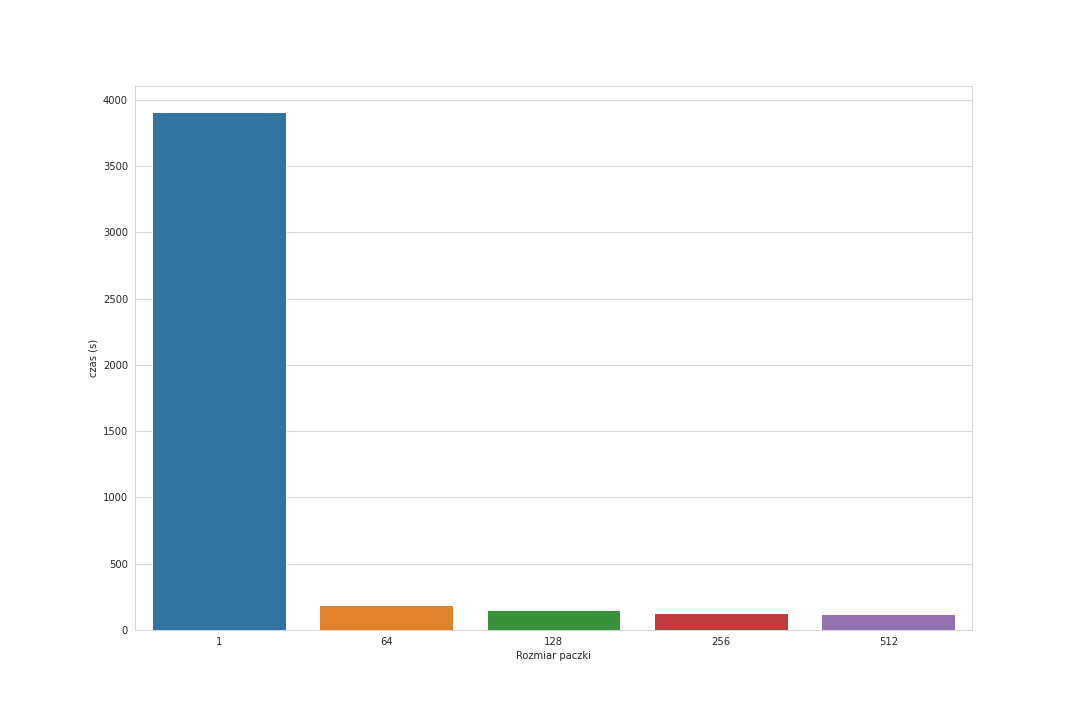
\includegraphics[width=\textwidth]{images/batch_size_time.png}
  \caption{Wielkość paczki równa 1}
\end{figure}

\subsection{Przedział inicjalizacji wag}
Wagi sieci neuronowej muszą być zainicjalizowane losowo, w przeciwnym wypadku uczenie byłoby niemożliwe.
Sieci, których wagi początkowe były z małymi odchyleniami standardowymi cechowały się szybszym tempem zbiegania.
Inicjalizacja wag jest szczególnie ważna w przypadku, w którym sieci wielowarstwowych.
Dobra inicjalizacja pomaga przeciwdziałać problemom zanikających i eksplodujących gradientów.
\begin{figure}[H]
  \centering
  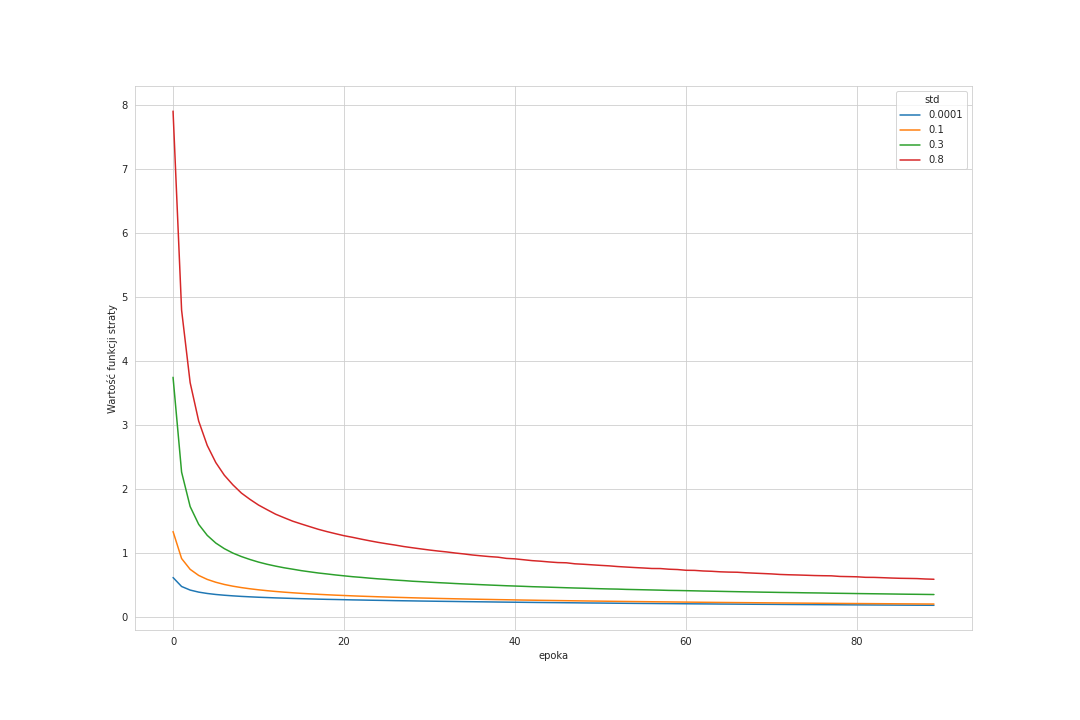
\includegraphics[width=\textwidth]{images/std_comp.png}
  \caption{Wpływ przedziału inicjalizacji wag}
\end{figure}

\begin{figure}[H]
  \centering
  \subfloat{{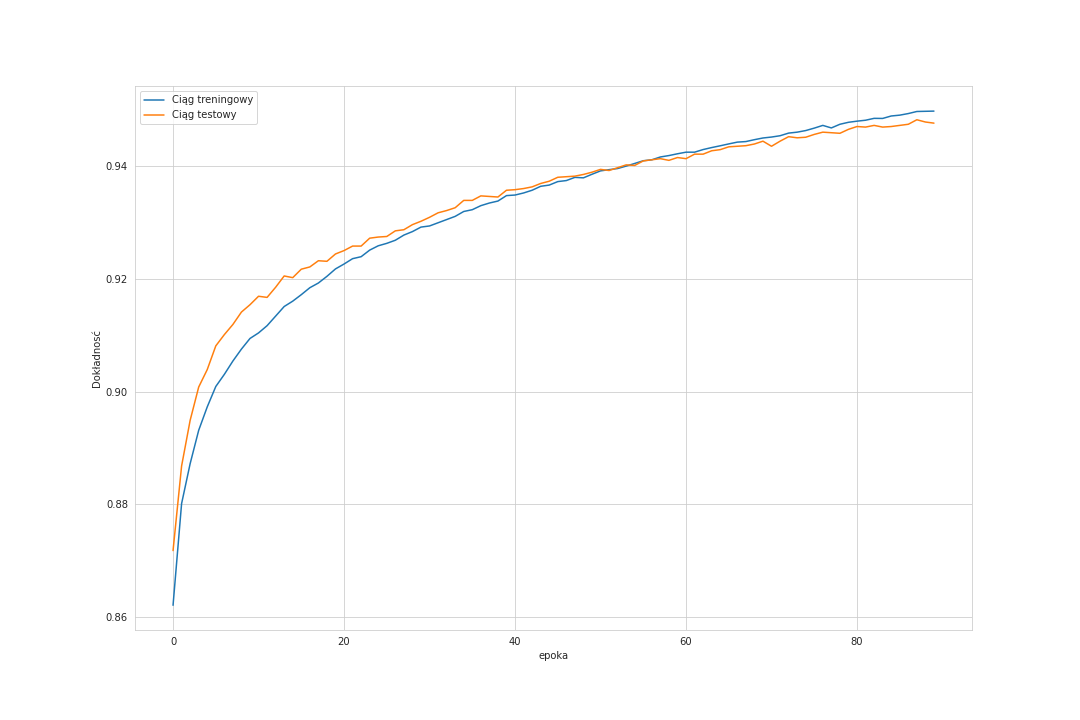
\includegraphics[width=0.45\textwidth]{images/std_0001_accuracy.png} }}
  \subfloat{{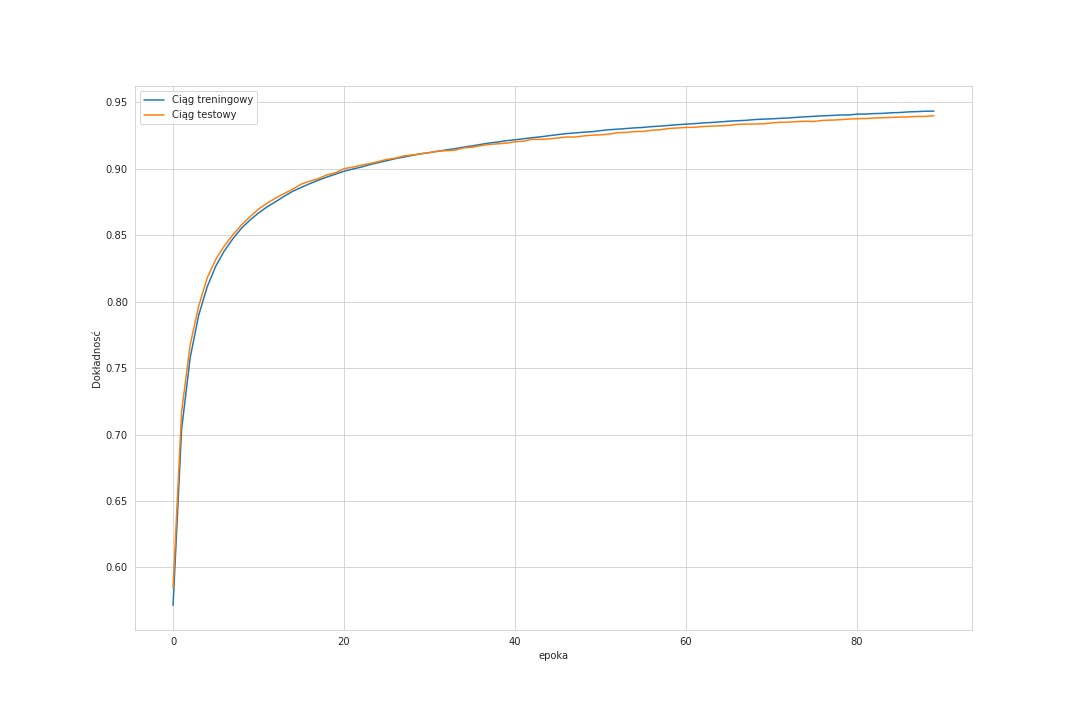
\includegraphics[width=0.45\textwidth]{images/std_01_accuracy.png} }}
\caption{Porównanie dokładności na ciągu treningowym i testowym dla odchyleń standardowych 0.0001 i 0.01}
\end{figure}

\pagebreak
\subsection{Funkcja aktywacji}
Funkcja aktywacji pozwala sieci na nauczenie się zależności nieliniowych.
Zbadano wpływ, jaki mają funkcje: sigmoidalna, tangens hiperboliczny oraz ReLU (rectified linear unit).
Funkcja sigmoidalna była tradycyjnie wykorzystywana podczas uczenia sieci neuronowych, ponieważ pomagała przeciwdziałać problemowi eksplodujących gradientów.
Jej głowną wadą jest niemalże "płaska" pochodna dla małych i dużych wartości wejścia.
Gradient funkcji jest niezerowy tylko w okolicach zera, z tego powodu, sieci z aktywacją sigmoidalną często cierpią na problem zanikającego gradientu.
Obecnie najcześciej wykorzystywaną funkcją jest funkcja ReLU, która 
znacznie ułatwia uczenie głębokich sieci neuronowych. Kolejną zaletą jest bardzo mały koszt obliczeniowy. 

Co ciekawe, zarówno sigmoida, jak i tangens hiperboliczny są obecnie częściej spotykane jako część komórki LSTM (long short-term memory).

Zgodnie z oczekiwaniami, funkcja ReLU osiągnęła znacznie lepszy wynik od tangensa hiperbolicznego i sigmoidy.
\begin{figure}[H]
  \centering
  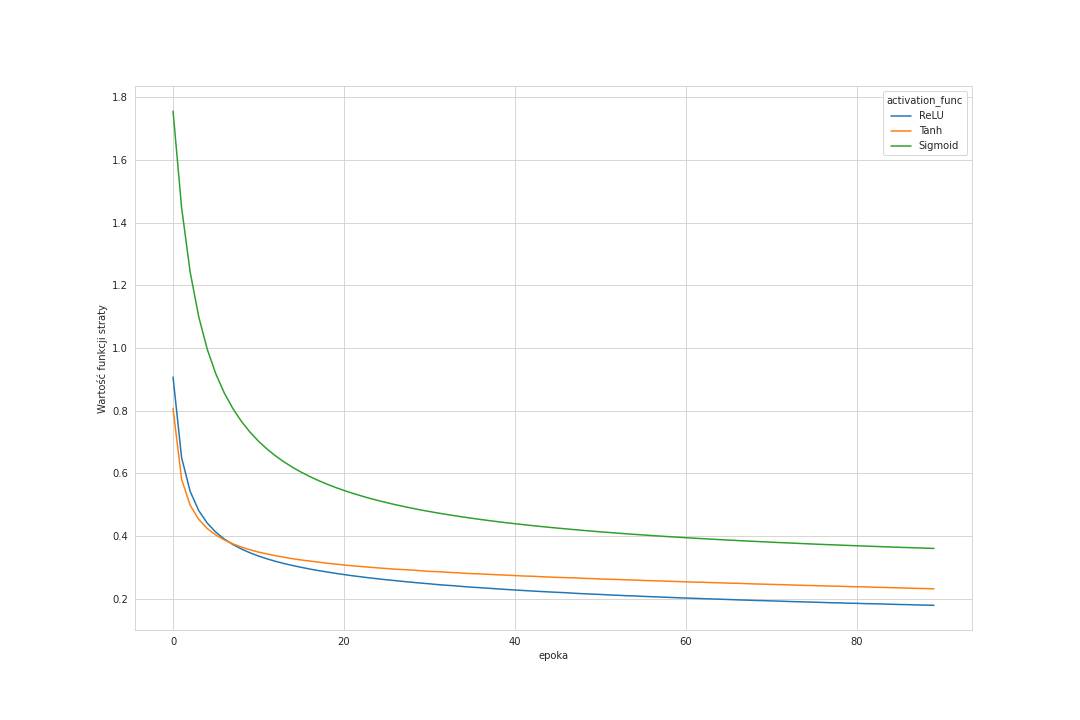
\includegraphics[width=\textwidth]{images/act_func_comp.png}
  \caption{Wpływ rodzaju funkcji aktywacji}
\end{figure}

\pagebreak
\section{Sprawdzanie gradientu}
Zaimplementowano algorytm aproksymacji numerycznej gradientu, za którego pomocą można sprawdzić poprawność implementacji propagacji wstecznej. 
Ze względu na dużą złożoność obliczeniową, algorytm nie nadaje się do wykorzystania podczas uczenia.
\begin{figure}[H]
  \centering
  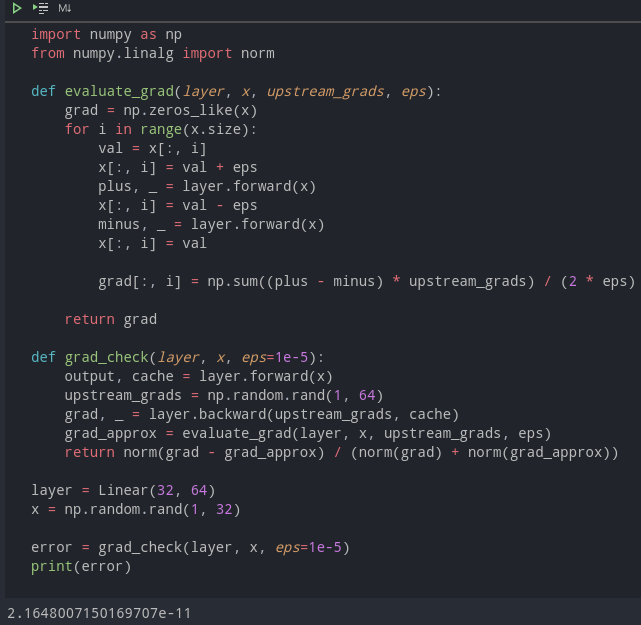
\includegraphics[width=\textwidth]{images/grads.png}
  \caption{Algorytm sprawdzania gradientu}
\end{figure}


\section{Wnioski}
Liczba neuronów w warstwie ukrytej decyduje o złożoności modelu.
Zbyt duża liczba neuronów prowadzi do przeuczenia oraz wpływa negatywnie na
czas uczenia.
Wykorzystanie dużego modelu ma sens w przypadku, w którym dysponujemy
dużym zbiorem danych oraz zależy nam na jak najwyższej dokładności predykcji.

Mini-batch gradient descent to kompromis pomiędzy algorytmem gradientu stochastycznego a wykorzystaniem całej epoki.
Wielkość paczki nie może być za duża, ponieważ oznacza to zbyt wolną aktualizację wag modelu, ani zbyt mała, co może skutkować zbyt dużym szumem.
W praktyce, o rozmiarze paczki decyduje najczęściej dostępna pamięć karty graficznej.

W przypadku funkcji aktywacji, zdecydowanym faworytem okazała się funkcja ReLU, 
która pozytywnie wpłynęła na szybkość uczenia.
Wybór funkcji aktywacji ma szczególne znaczenie podczas uczenia
głębokich sieci, ze względu na problemy zanikających oraz eksplodujących 
gradientów.

Wagi modelu zostały zainicjalizowane z rozkładu normalnego.
Najbardziej korzystny wpływ na szybkość uczenia miały małe wartości, skupione w zerze.
Wybranie zbyt małej wartości odchylenia standardowego będzie skutkowało szybkim zaniknięciem gradientów i brakiem aktualizacji wag, przez co uczenie będzie nieskuteczne.

Współczynnik uczenia jest ważnym parametrem, który bezpośrednio wpływa 
na szybkość uczenia.
Zbyt duża wartość będzie powodowałą problemy ze zbieżnością, a za mała, długi czas uczenia.
Dobrym pomysłem jest wykorzystanie zmiennego współczynnika uczenia, co pozwoli
połączyć zalety dużego współczynnika na początku treningu, z zaletami mniejszego
w dalszym etapie uczenia.



\end{document}


Poni¿ej znajduje siê tabela, w której znajduj¹ siê informacje jak zapisaæ poprawnie polskie znaki w formie zakodowanej:
POLSKA LITERA   KOD TEX POLSKA LITERA   KOD TEX
¹       \k{a}   ¥       \k{A}
æ       \'c     Æ       \'C
ê       \k{e}   Ê       \k{E}
³       \l{}    £       \L{}
ñ       \'n     Ñ       \'N
ó       \'o     Ó       \'O
œ       \'s     Œ       \'S
¿       \.z     ¯       \.Z
Ÿ       \'z            \'Z

